\graphicspath{{images/}}

\section{Methods}
\label{sec:methods}

\subsection{CANS}

I developed a Python package (CANS) for model composition, model
simulation, parameter inference, and visualisation of results. I use
CANS to fit the competition model to QFA data. CANS accepts cell
density timecourses for locations in rectangular arrays of arbitrary
size. SBML models are produced to document results of parameter
inference, and for independent validation using other simulation
tools. It is simple to create new models with reactions which are
common to each location, including diffusion reactions between nearest
neighbours. CANS is available at:
\href{https://github.com/lwlss/CANS}{https://github.com/lwlss/CANS}.

% \subsection{\thesubsection~Description of datasets}

\subsection{The P15 dataset}
\label{sec:P15_description}

I compared the logistic and competition model by fitting both to a
single plate from a previous QFA study on \textit{S. Cerevisiae}
\citep{Addinall2011}. I call this plate P15. A 3x3 section is shown in
Figure~\ref{fig:p15_section}. P15 contains 384 cultures, all with
background mutation \textit{cdc13-1}. \textit{cdc13} is involved in
telomere stability and \textit{cdc13-1} is a temperature-dependent
mutation. Each culture also has a deletion from a standard deletion
library containing 49 different deletions thought to affect telomere
function. There are 6 repeats of each of these deletions. There are
also 14 repeats of a strain with a neutral deletion,
\textit{his3}\(\Delta\). Edge cultures are inoculated with extra
repeats of the neutral deletion, but results are discarded due to
noise from reflections off plate walls. Inoculum density is
\(\sim\)100 cells, which is below the level of detection. P15 was
incubated at 27\(^{\circ}\)C, at which point \textit{cdc13-1} starts
to experience loss of function. Each culture has a cell density
timecourse with 10 timepoints covering 4 days. Several features make
P15 a good test case. Strains vary greatly in fitness, so competition
should be present. Repeats of each strain increase statistical
power. Furthermore, for several strains, independent spot tests have
been published and may be used for validation
\citep{maringele2002exo1,zubko2004exo1,Holstein20141259,foster2006mrx}.

\subsection{The Stripes and Filled datasets}
\label{sec:stripes_description}

I used a two-plate QFA experiment (E. Holstein, personal
communication, April 2016) to validate the competition model. Images
of the plates, termed the ``Stripes'' and ``Filled'' plates, are shown
in Figure~\ref{fig:stripes_images}. As for P15, the experiment uses
strains of \textit{S. Cerevisiae} with a background mutation, and a
deletion in a gene relevant to telomere function. In contrast to P15,
there are more deletions per plate and no repeats for most
strains. Identical strains are repeated in the same positions on each
plate, except in every second column in the Stripes plate, where
locations are left empty. The common cultures have background mutation
\textit{cdc13-1}, as used in P15, and identical strains are inoculated
from the same liquid culture to reduce genetic variation. The extra
columns in the Filled plate are a transposition of the columns to the
left, but with a different query mutation
\textit{rad75}\(\Delta\). The leftmost column in the Filled plate
contains repeats of the neutral deletion,
\textit{his3}\(\Delta\). Inoculum density is \(\sim\)10,000 cells,
which is much higher than that used in P15, and detectable at time
zero. The plates were incubated together at 27\(^{\circ}\)C, where the
defect of \textit{cdc13-1} is larger than that of
\textit{rad75}\(\Delta\).  Each culture has a cell density timecourse
with \(\sim\)50 timepoints covering four days. This is about five
times as many timepoints as collected for P15.

% This might get repeated in the results.
The different neighbour configurations cause identical strains to grow
differently between the two plates. To validate the competition model,
I calibrate parameters on the Filled plate and validate by simulating
timecourses for the Stripes plate. This is possible because the Filled
plate contains all of the strains present on the Stripes plate.

\subsection{Solving and fitting}

\subsubsection{Solving}
\label{sec:solving_comp}

CANS solves ODE models numerically using one of two packages:
integrate from SciPy, and libRoadRunner. The method integrate.odeint
solves ODEs written in Python, at user supplied timepoints. I used
NumPy to vectorise competition model ODEs to optimise solving by this
method. libRoadRunner is implemented in C++ and solves ODEs for models
written in SBML. I access libRoadRunner through its Python API, and
use the libSBML Python API to automatically generate SBML versions of
the competition model for any size plate. For a 16x24 culture plate
with cell density observations at 10 evenly spaced timepoints,
libRoadRunner is approximately 10 times faster than SciPy's integrate,
solving in hundredths rather than tenths of a second. Unlike SciPys's
integrate.odeint, libRoadRunner solves only at evenly spaced
timepoints. To fit P15, where each timecourse has 10 unevenly spaced
timepoints, I simulated sequentially between adjacent timepoints. For
the Stripes and Filled plates, which have \(\sim\)50 unevenly spaced
timepoints, I sampled 15 evenly spaced timepoints from a spline. I use
SciPy's interpolate.splrep to make 5th order B-splines with smoothing
condition \(s=1.0\), and SciPy's interpolate.splev to evaluate. The
sampled timepoints range from time zero to the time of last
observation. Solving then requires just one call to libRoadRunner's
RoadRunner.simulate. Using libRoadRunner on a modern CPU, fitting a
16x24 format plate with 10 unevenly spaced timepoints takes \(\sim\)3
hours; fitting a full plate with 15 evenly spaced timepoints takes
\(\sim\)1 hour.

\subsubsection{Fitting the competition model}
\label{sec:fitting_comp}

I processed raw QFA data using Colonyzer \citep{Lawless2010} to
produce cell density timecourses.
% I use QFA data after processing with Colonyzer \citep{Lawless2010}.
% Colonyzer uses integrated optical density measurements in whole plate
% images as a proxy for cell density. I used timecourse cell density
% estimates, which have arbitrary units, throughout my analysis.
To these, I fit the competition model, using a gradient method, and
normal model of measurement error, to make maximum likelihood
estimates of parameters. The particular gradient method was a
constrained minimisation: the L-BFGS-B algorithm from SciPy's
integrate package. I determined stopping criteria so that parameters
of simulated full-plate data sets, with a small amount of simulated
noise, were recovered with high precision. To help the minimizer, I
scaled \(C(0)\) values by a factor of \(10^{5}\) to make them closer
to other parameter values. For each plate, I ran many fits with
different initial parameters to try to find a global minimum (see
Sections~\ref{sec:P15_fit} and \ref{sec:cross_plate_val_results}). I
set parameter bounds according to Table~\ref{tab:p15_bounds}, and
checked that best fits had no parameters at a boundary.

\begin{center}
  \captionof{table}{\textbf{Parameter bounds for fitting the
      competition model to P15 and the Stripes and Filled plates.}
    The same bounds on \(N(0)\) were used for both internal and edge
    cultures. Bounds on \(C(0)\) and \(N(0)\) were set using initial
    conditions: ``guess'' refers to the initial guess of each
    parameter (see Section~\ref{sec:initial_guess}).}
  \begin{tabular}{| c | c c |}
    \hline
    Parameter        & Lower Bound  & Upper Bound \\
    \hline
    \(C(0)\)     & guess x \(10^{-3}\)  & guess x \(10^{3}\)\\
    \(N(0)\)     & guess / \(2\)  & guess x \(2\)\\
    % \(N^{I}(0)\) \& \(N^{E}(0)\) & guess / \(2\)  & guess x \(2\)\\\\
    \(k\)        & 0.0    & 10.0\\
    % \(b\) (all cultures)           & 0.0    & \(\infty\) \\
    \(b\)           & 0.0    & None \\
    \hline
  \end{tabular}
  \label{tab:p15_bounds}
\end{center}

Cultures at the edge of a plate gain an advantage from accessing a
greater area of nutrients. I corrected for this using separate
parameters, \(N_{I}(0)\) and \(N_{E}(0)\), for the initial amount of
nutrients in internal and edge cultures. In rate equations involving
edge cultures, I scaled edge culture nutrient amount by the ratio
\(N_{I}(0)/N_{E}(0)\). The physical interpretation of this correction
is that edge cultures have an extra supply of nutrients that can
diffuse instantly into the reaction volume. This treatment increased
the closeness of fit to cultures one row or column inside the edge,
and to internal cultures overall (see Table~\ref{tab:corner} in
Section~\ref{sec:treatment_of_boundaries}). Cell density measurements
from edge cultures contain extra noise due to reflections from plate
walls \citep{Lawless2010}. For the competition model, unlike the
logistic model, these cannot simply be discarded prior to
fitting. Instead, I collectively fit to all cultures and selected best
fits based on only the closeness of fit to internal cultures.

% %%%% Empties %%%%%
% (Can go to results section or Stripes method section:) QFA data for
% the Stripes plate contained observations for cultures that were known
% to be empty. When fitting the competition model, I set growth constant
% \(b\) to zero for these cultures and removed them from fitting.
%%%% End Empties %%%%%

\subsubsection{Fitting the logistic model}

Fitting the mass action logistic model requires a culture level
\(N(0)\), creating 383 extra parameters. The QFA R package
\citep{qfa2016} can fit the standard logistic model, and has heuristic
checks to correct a confounding of \(r\) and \(K\) parameters that
occurs when slow-growing cultures are dominated by noise. I did not
have time to implement these checks for the mass action logistic
model, so I instead fit using the QFA R package. This is not
equivalent to the competition model fit because the QFA R package uses
a culture level \(C(0)\), i.e.,~there is no collective fitting. This
makes 1152 total parameters, rather than the 769 that we would have
using the mass action logistic model. It is, nevertheless, useful to
compare fitting of the competition model with the standard logistic
model from the QFA R package, because the latter has been used in
previous QFA papers, including \citet{Addinall2011} from which we take
P15.
% I do not expect much disagreement of fitness estimates with the mass
% action logistic model once heuristic checks are implemented.
In contrast to the competition model, noisy data from edge cultures
can be discarded prior to fitting the logistic model.

\subsubsection{Data visualisation}

I used the Python package matplotlib to create plotting functions in
CANS to visualise fits and simulations of QFA timecourses and to
compare the ranking of fitness estimates.

\subsection{Parameter conversion}
\label{sec:parameter_conversion}

In the independent limit (\(k=0\)), it is possible to equate \(C\) of
the competition and logistic model. Parameters can then be converted
as follows:
% When \(k\) is set to zero, the competition model
% (\ref{eq:competition_model}) reduces to the mass action logistic model
% which has the same sigmoidal solution as the standard logistic
% model. In this limit, it is possible to equate C species of both
% models and convert parameters using,
% Derivation or link to blog.
\begin{subequations}
  \label{eq:conversion}
  \begin{align}
    &r = b(C(0) + N(0)),\\
    &K = C(0) + N(0).
    % &r = b(C(0) + N(0))\\
    % &K = (C(0) + N(0))
  \end{align}
\end{subequations}
%
The competition model assumes that all nutrients are converted to
cells, implying that all cultures starting with the same amount of
nutrients reach the same final amount of cells. As final cell amounts
generally differ, it is, therefore, necessary to allow \(N(0)\) to
vary for each culture when fitting the mass action logistic
model. This is not realistic; the competition model already assumes
\(k>0\). It is, nevertheless, possible to disregard our interpretation
of the competition model, fit the mass action logistic model, and
convert parameters to those of the standard logistic model. This is
illustrated in Figure~\ref{fig:correction}a showing a single culture
from a 16x24 format plate. This culture grew faster than its
neighbours (not shown) and reached a higher final cell amount. Notice
that estimated \(N(0)\) is approximately equal to final cells. The
conversion equations can also be used to return corrected \(r\) and
\(K\), for growth in independent conditions, after first fitting the
full competition model. This is illustrated in
Figure~\ref{fig:correction}b, in a fit to the same culture, where
dashed lines represent the corrected fit.
% resimulated with \(k=0\)
Notice that corrected values of \(r\) and \(K\) differ from those in
Figure~\ref{fig:correction}a.


% Figure~\ref{fig:correction} shows fits of a single culture on a larger
% 16x24 format plate using both models. This culture grew faster than
% its neighbours (not shown) and, according to the competition model,
% competed for more nutrients.
% %
% Figure~\ref{fig:correction}a shows the mass action logistic model fit
% where \(N(0)\) is estimated as being approximately equal to the final
% cell amount, or equivalently, carrying capacity \(K\).
% %
% Figure~\ref{fig:correction}b shows the competition model fit with a
% plate level \(N(0)\) and \(k > 0\). Re-simulating with \(k\)
% set to zero gives the dashed mass action logistic model curves which
% are corrected for competition. We can therefore obtain the corrected
% logistic model \(r_{i}\) and \(K_{i}\) of these curves by converting
% from competition model estimates of \(b_{i}\), \(C(0)\), and
% \(N(0)\).
% N.B. \(b\) is the same for both the solid and dashed
% curves in Figure~\ref{fig:correction}b.
% This produces the correction in \(r\) and \(K\) between the two fits
% (see Figures~\ref{fig:correction}) and allows direct comparison
% between competition and logistic model estimates.

It is easy to compare competition model \(b\) with logistic model
parameters, because \(C(0)\) and \(N(0)\) are fit collectively for
each plate. This leads to \(b \propto r \propto MDR\) (see
Equations~\ref{eq:MDR_MDP} and \ref{eq:conversion}). Note also that
all cultures have the same \(K\) and \(MDP\). \(b\) is therefore
equivalent to several common QFA fitness measures: \(r\), \(MDR\), and
\(MDR*MDP\) \citep{Addinall2011}. This makes \(b\) a very convenient
fitness measure; we need not convert to logistic model parameters to
compare the fitness rankings of cultures on the same plate. To compare
fitness rankings between different plates we can of course use
\(b\). This is not, however, equivalent to comparing \(r\) or \(MDR\)
as different plates may have different \(C(0)\) and \(N(0)\).

% Competition model \(C(0)\) and \(N(0)\) are the same for all cultures
% on a plate. Therefore, by the conversion equations
% (\ref{eq:conversion}), all cultures on a plate have the same carrying
% capacity \(K\) and all \(b_{i} \propto r_{i}\) by the same
% factor. Similarly, \(MDP\) is the same for all cultures and all
% \(b_{i} \propto MDR_{i}\) by the same factor (see
% Equation~\ref{eq:MDR_MDP}). Therefore, \(b\) is equivalent to common
% QFA fitness measures, \(r\), \(MDR\), and \(MDR*MDP\) (see
% e.g. \citet{Addinall2011}). This makes \(b\) a very convenient fitness
% measure for the competition model; we need not convert to logistic
% model parameters to compare the fitness rankings of cultures on the
% same plate. To compare competition model fitness rankings between
% different plates we can of course use \(b\). However, this is not
% equivalent to comparing \(r\) or \(MDR\) as different plates may have
% different \(C(0)\) and \(N(0)\).

\begin{Figure}
  \centering
  \graphicspath{{images/correction/}}
  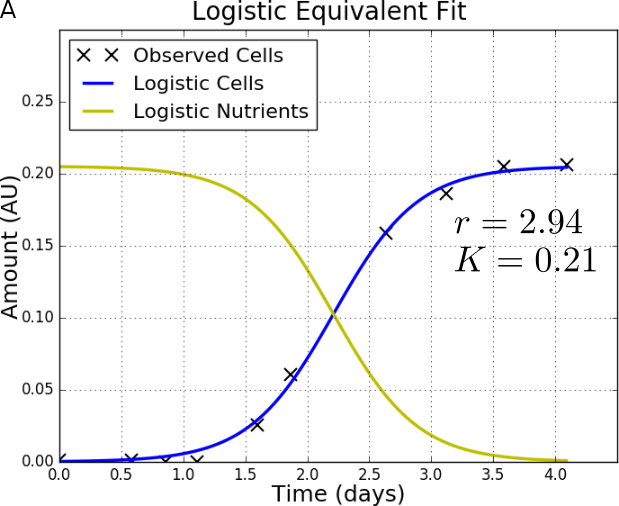
\includegraphics[width=\linewidth]{final/logisticA}
  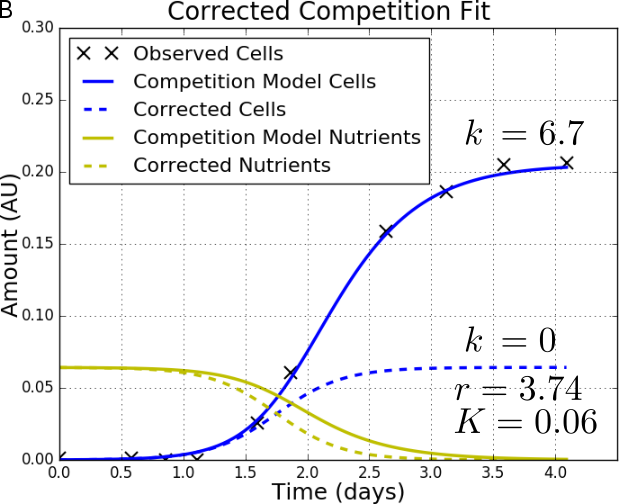
\includegraphics[width=\linewidth]{final/competitionB}
  \captionof{figure}{\textbf{Using the competition model to return
      logistic model parameters.} \textbf{A)} Fit of the mass action
    kinetic model displaying \textbf{converted} logistic model
    parameters. \textbf{B)} Fit of the full competition model (solid;
    \(k=6.7\)), and simulation of independent growth (dashed; \(k=0\))
    displaying \textbf{corrected} logistic model parameters. Both fits
    are to culture (R10, C3) of P15 which grew faster and reached a
    higher final cell density than its neighbours (not shown).}
    % According to the competition model, this is because this
    % culture competed for more nutrients. To reach the same final cell
    % density, the mass action logistic model requires a higher amount
    % of starting nutrients for this culture and a different amount for
    % each neighbour. The correction to the competition model simulates
    % how growth would have appeared without competition and, for the
    % culture shown,
    % gives~\(r_{corrected} >
    % r_{logistic}\)~and~\(K_{corrected} < K_{logistic}\).
  \label{fig:correction}
\end{Figure}

\subsection{Determining initial parameters}
\label{sec:initial_guess}

Collectively fitting the competition model to a standard 384-format
QFA plate is a formidable optimisation problem involving 384
timecourses and 387 parameters. Achieving good fits therefore requires
making a good initial guess. To fit small simulated zones I could
simply use many random parameter guesses. However, for a full plate
the chance of any random guess being close to the ``true'' values
diminishes and more sophisticated guessing methods are required. I
developed the \textit{Imaginary Neighbour Model}
(Figure~\ref{fig:imag_neigh_schematic}) for guessing competition model
\(b_{i}\) and this allowed good fits of to be made. As the project
progressed, it became clear how to convert between fast logistic
parameter estimates and competition model parameters (see
Section~\ref{sec:parameter_conversion}) and this could be a valid
alternative.

\subsubsection{Guessing initial amounts}
\label{sec:guessing_amounts}

Recall from the competition model reaction equations
(\ref{eq:reaction} and \ref{eq:diffusion_reaction}) that nutrients can
only diffuse or be converted to cells. Thus, assuming that reactions
are nearly complete at the end of cell observations and that
\(C(0) \ll C(\infty)\), the total initial amount of nutrients,
\(N_{Tot}\), can be estimated using,
\begin{equation}
  \label{eq:N_Tot}
  N_{Tot} = n_{I}N_{I}(0) + n_{E}N_{E}(0) \approx C_{F},
\end{equation}
where \(C_{F}\) is the total of final cell measurements, \(n_{I}\) and
\(n_{E}\) are the numbers of internal and edge cultures, and
\(N_{I}(0)\) and \(N_{E}(0)\) are initial nutrient amounts
for internal and edge cultures (see
Section~\ref{sec:fitting_comp}). Using (\ref{eq:N_Tot}), and an estimate
for the ratio of area associated with edge cultures to area associated
with internal cultures,
\(A_{r} = A_{E} / A_{I} = N_{E}(0) / N_{I}(0)\), I made
guesses of \(N_{I}(0)\) and \(N_{E}(0)\) using,
%
\begin{equation}
  \label{eq:N_0_guesses}
  \begin{aligned}
    % &A_{r} = A_{E} / A_{I} = N_{E}(0) / N_{I}(0)\\
    % &N_{Tot} = n_{I}N_{I}(0) + n_{E}N_{E}(0) \approx C_{F}\\
    &N_{I}(0) = N_{Tot} / (n_{I} + n_{E}A_{r})\\
    &N_{E}(0) = N_{Tot} / (n_{I}/A_{r} + n_{E}).
    % &N_{E}(0) = (N_{Tot} - n_{I}N_{I}(0)) / n_{E}.
  \end{aligned}
\end{equation}
%
When \(A_{r} = 1\), (\ref{eq:N_0_guesses}) reduces to the initial
nutrient guess for the one initial nutrient parameter model. I used
\(A_{r} = 1.5\).

In QFA using dilute cultures, \(C(0)\) falls below the level of
detection. I did not estimate initial guesses of \(C(0)\) and instead
ran multiple fits over a range of \(C(0)\) values in logspace chosen
to encompass uncertainty in \(C(0)\) for the given experiment. I
expressed this as a ratio, \(C_{r}\), multiplied by the initial
nutrient guess \(N(0)_{I}\).

% ; for P15 \(10^{-5}\) to \(10^{-3}\) times the
% average final cell amount, for the Stripes and Filled plates
% \(10^{-7}\) to \(10^{-1}\) times average final cell amount.


\subsubsection{\boldmath Guessing \(b\) \unboldmath}
\label{sec:guessing_b}
%%%%%%%%%%%%%%% Imag neigh %%%%%%%%%%%%%%%%%%%

\graphicspath{{images/imag_neigh_schematic/}}
\begin{Figure}
  \centering
  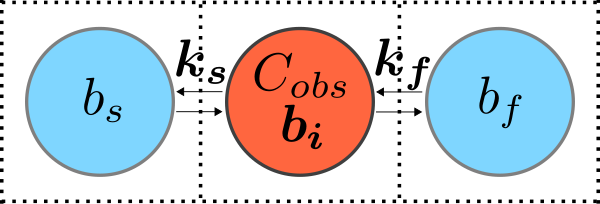
\includegraphics[width=\linewidth]{final/imag_neigh_schematic_2}
  \captionof{figure}{\textbf{Schematic of the imaginary neighbour
      model.} I developed this model to make quick guesses of
    competition model \(b_{i}\) by fitting single cultures. A real
    culture (red) with cell observations, \(C_{obs}\), is modelled as
    growing alongside imagined slow and fast growing neighbours (blue)
    with growth constants \(b_{s}\) and \(b_{f}\) (for slow and
    fast). The model uses separate nutrient diffusion constants
    \(k_{s}\) and \(k_{f}\) for slow and fast growing neighbours
    rather than a single parameter \(k\). \(k_{s}\), \(k_{f}\), and
    the growth constant \(b_{i}\) of the real culture are estimated by
    fitting the model to \(C_{obs}\) with all other parameters
    fixed. Different numbers of each neighbour can be chosen to
    replicate different configurations of neighbours that might be
    present on a real plate.}
  \label{fig:imag_neigh_schematic}
\end{Figure}

% The model aims to approximate the diffusion of nutrients into and out
% of a culture using an configuration of imagined fast and slow growing
% neighbours. Cell observations for a culture can be fit to get
% estimates of growth constants \(b_{i}\).\\

To guess competition model \(b_{i}\) I used the imaginary neighbour
model (Figure~\ref{fig:imag_neigh_schematic}) to quickly fit
individual cultures. The model is based on the reaction and rate
equations of the competition
model~(\ref{eq:reaction}--\ref{eq:diffusion_reaction}) but tries to
replicate the diffusion of nutrients into and out of a culture using
imaginary fast and slow growing neighbours, with growth constants
\(b_{f}\) and \(b_{s}\), and different nutrient diffusion constants
\(k_{f}\) and \(k_{s}\). To fit the model to QFA data, I fixed
\(C(0)\) and \(N(0)\) for all cultures by the initial guesses (see
Section~\ref{sec:guessing_amounts}), I fixed \(b_{f}\) at a high value
and fixed \(b_{s} = 0\), I allowed \(b\), \(k_{f}\), and \(k_{s}\) to
vary with lower bound zero and no upper bound. I used initial values
of zero for \(k_{f}\) and \(k_{s}\). I carried out multiple fits of
the imaginary neighbour model for each value of \(C_{0}\), with
initial values for \(b\) taken from the range (35, 40, ..., 100) and
\(b_{f}\) fixed as 1.5 times this value. I determined the number,
\(n\), of each neighbour from the guess of \(N_{I}(0)\) and the range
of final cell amounts, such that the culture with the highest observed
final cell density had enough slow growing neighbours to provide all
of the nutrients necessary to reach this final cell density. I solved
the imaginary neighbour model using SciPy's odeint and fit using a
gradient method as in Section~\ref{sec:fitting_comp}. Fits of the
imaginary neighbour model take several minutes which is fast compared
to fits of the competition model which take on the order of hours.

%%%%%%%%%%%%%%% Imag neigh %%%%%%%%%%%%%%%%%%%%%%%%%%%%%%%%%%%%%%

\subsubsection{\boldmath Guessing \(k\) \unboldmath}

Simulations of the competition model using sets of \(b\) parameters
drawn from different normal distributions have linear relationships
between variance in final cell amount and nutrient diffusion constant
\(k\). I simulated guessed parameters \(C(0)\), \(N(0)\), and
\(b_{i}\) with a range of different \(k\) values and used linear
regression to parameterise the straight line. I then took the variance
in final cell amount for real data and used the regression model to
predict \(k\).
% \\\\
% Don't think I need this figure. r->b and make titles bigger. Fitted
% \(k\) was much higher so I should probably resimulate over a
% bigger range. Only possibly to know in hindsight. I could also use the
% fitted parameters for this rather than drawing from a normal
% distribution.
% \\
% \graphicspath{{images/guessing/}}
% \begin{Figure}
%   \centering
%   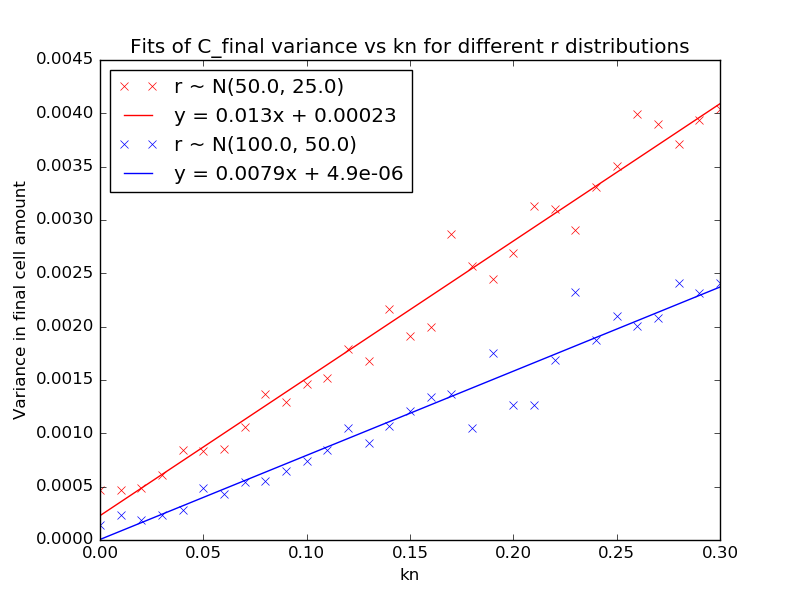
\includegraphics[width=\linewidth]{final/kn_guessing}
%   \captionof{figure}{\textbf{Guessing \(\bm{k}\) from the variance in
%       final cell amounts.} The competition model is simulated for a
%     16x24 format plate using two random sets of culture-level \(b\)
%     parameters drawn from different normal distributions. Each set of
%     \(b\) parameters is simulated with a range of \(k_n\) parameter
%     values. The variance in final cell density for all cultures is
%     plotted against \(k_n\) for each simulation. Lines are shown for
%     least squares fits to points from each set of \(b\) parameters.}
%   \label{fig:kn_guessing}
% \end{Figure}

% \subsection{\thesubsection~Development of a genetic algorithm}

% I began work on a hierarchical genetic algorithm method of parameter
% inference inspired by the hierarchical Bayesian analysis of QFA data
% by \citet{Heydari2016}. (I'm not sure that it is too similar or was in
% fact inspired by this.)

% p15 cell ratios
% cell_ratios = np.logspace(-3, -5, num=5)

% stripes and filled cell ratios
% cell_ratios = np.logspace(-1, -7, num=10) I increased the range to
% account for higher inoculum density and work of Herrmann.
%
% Results \(C(0)\), \(N_{I}(0)\), \(N_{E}(0)\), \(k\)
% est_params Stripes [ 0.00831517,  0.08524787,  0.09564223,  1.92525936]
% est_params Filled [ 0.00617039,  0.11660628,  0.1830217 ,  4.84354755]


%%% Local Variables:
%%% mode: latex
%%% TeX-master: "report"
%%% End:
